\documentclass[a4paper,UTF8]{article}
\usepackage{CJKutf8}
\usepackage[margin=1.25in]{geometry}
\usepackage{color}
\usepackage{graphicx}
\usepackage{amssymb}
\usepackage{amsmath}
\usepackage{amsthm}
\usepackage{multirow}
\usepackage{pdfpages}
\usepackage{tikz}
\usepackage{listings}
\usepackage{xcolor} 
\usepackage{longtable}
\usetikzlibrary{arrows,automata} 
\usepackage{algorithm}
\usepackage{algorithmic}
\renewcommand{\algorithmicrequire}{ \textbf{Input:}} %Use Input in the format of Algorithm
\renewcommand{\algorithmicensure}{ \textbf{Output:}} %UseOutput in the format of Algorithm

%\setmainfont                    [Ligatures=TeX]{Times New Roman}
\theoremstyle{definition}
\newtheorem*{solution}{Solution}
\newtheorem*{prove}{Proof}

\lstset{
	numbers=left, 
	numberstyle=\tiny,
	frame=shadowbox, 
	breaklines=true, 
	showspaces=false,
 	keywordstyle=\color{purple}\bfseries,
	%identifierstyle=\color{brown!80!black},
 	commentstyle=\color{gray}
	stringstyle=\color{brown!60!black},
	rulesepcolor=\color{red!20!green!20!blue!20}
}
\begin{document}
\begin{CJK}{UTF8}{gkai}
\title{大数据处理综合实验-实验2实验报告}
\author{
    小组15
}
\date{}
\maketitle

\begin{CJK*}{UTF8}{gbsn}
\section*{一、JAR包执行方式}
\end{CJK*}
	\par 说明:本次实验我们把所有功能打包在一个jar包内,通过指定主类选择功能。假定jar包的位置在lab2/lab2.jar位置。
	\par 注意:选做功能1(排序)在执行时需要以基础功能的输出作为输入,请确保执行前已经执行过倒排索引。
	\par 基础功能(倒排索引):
	\par hadoop jar lab2/lab2.jar InvertedIndexer $input\_path$ $output\_dir\_1$
	\par 选做功能1(排序):
	\par hadoop jar lab2/lab2.jar SortedCounter $output\_dir\_1$ $output\_dir\_2$
	\par 选做功能2(TF-IDF):
	\par hadoop jar lab2/lab2.jar TFIDF $input\_path$ $output\_dir\_3$

\begin{CJK*}{UTF8}{gbsn}
\section*{二、实验结果及输出文件路径}
\end{CJK*}
\begin{enumerate}
	\item[1.] 基础功能
	\par 输出文件路径:/user/2021sg15/lab2/out1
	\begin{figure}[H]
	    \centering
	    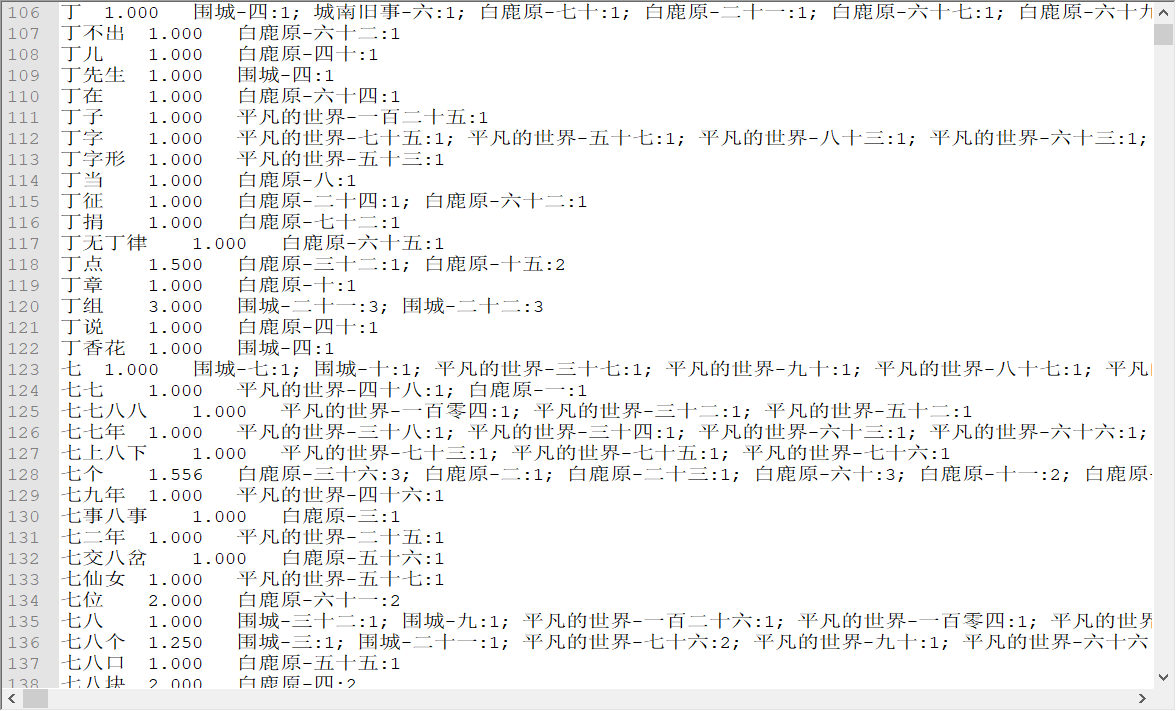
\includegraphics[scale=0.6]{./img/InvertedIndex_res.png}
	    \caption{基础功能-结果文件部分截图}
	\end{figure} 
	\begin{figure}[H]
	    \centering
	    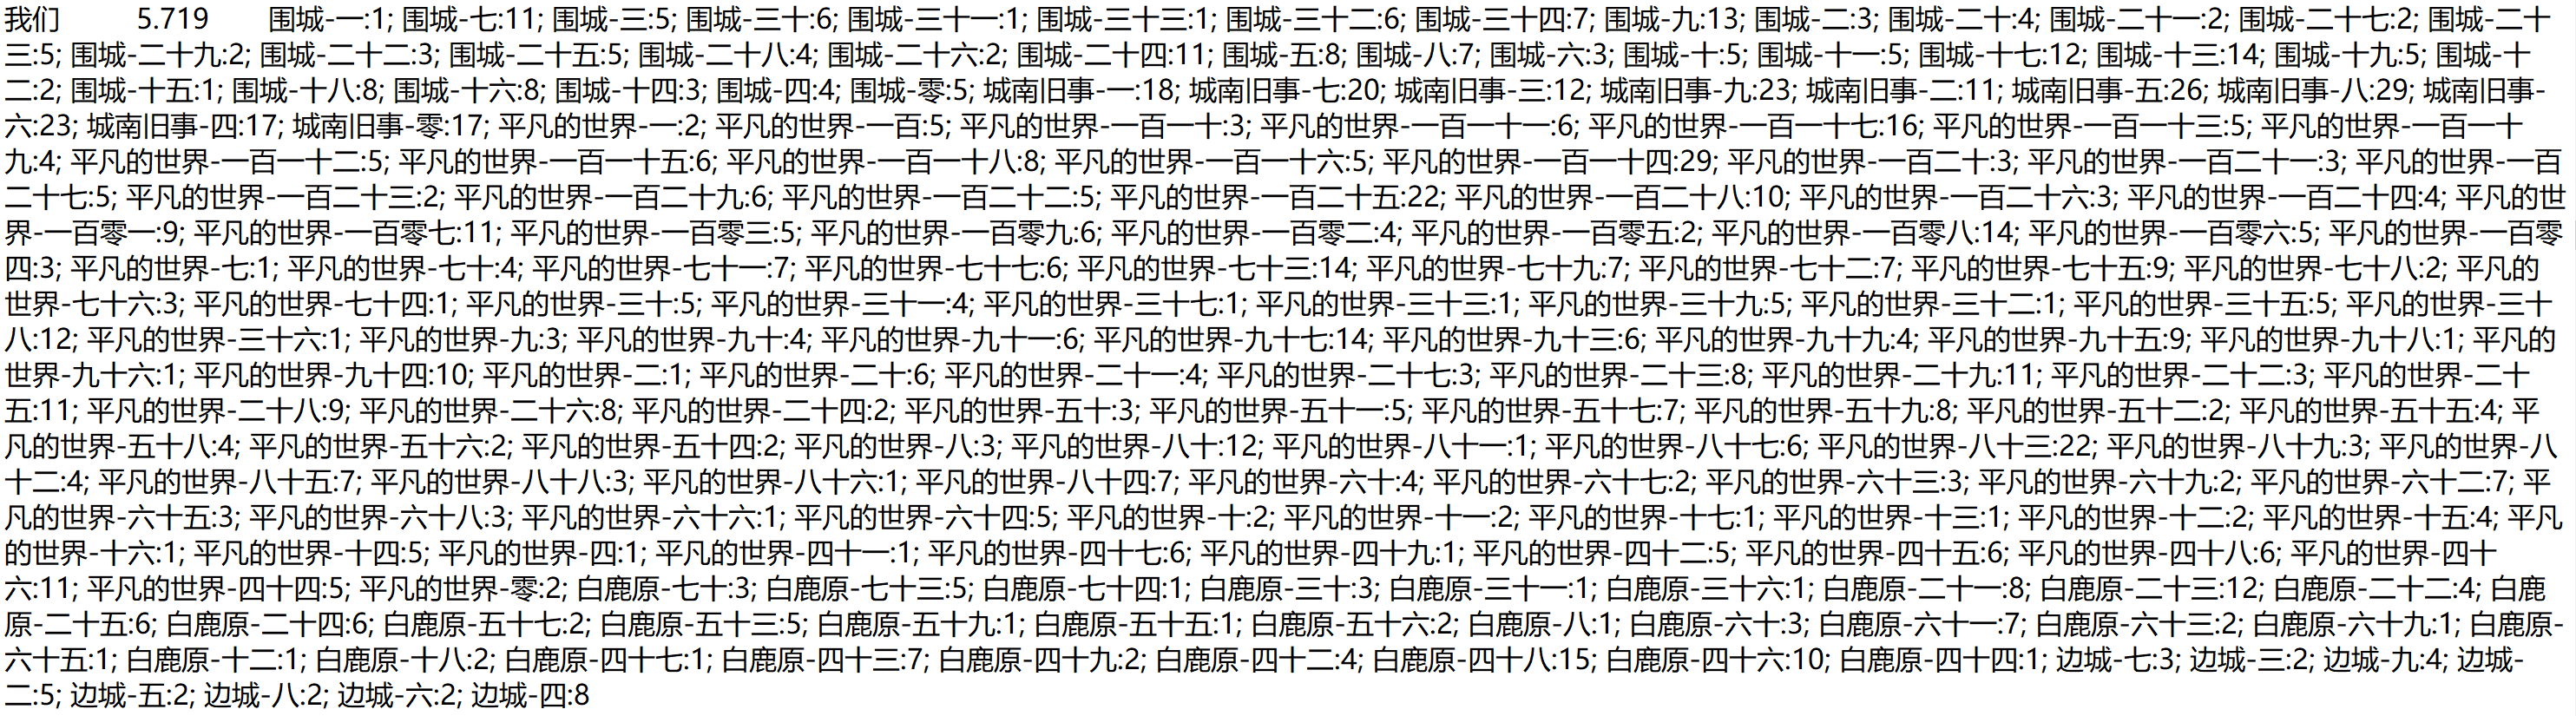
\includegraphics[scale=0.4]{./img/InvertedIndex_we.png}
	    \caption{基础功能-结果文件-“我们”}
	\end{figure} 
	\begin{figure}[H]
	    \centering
	    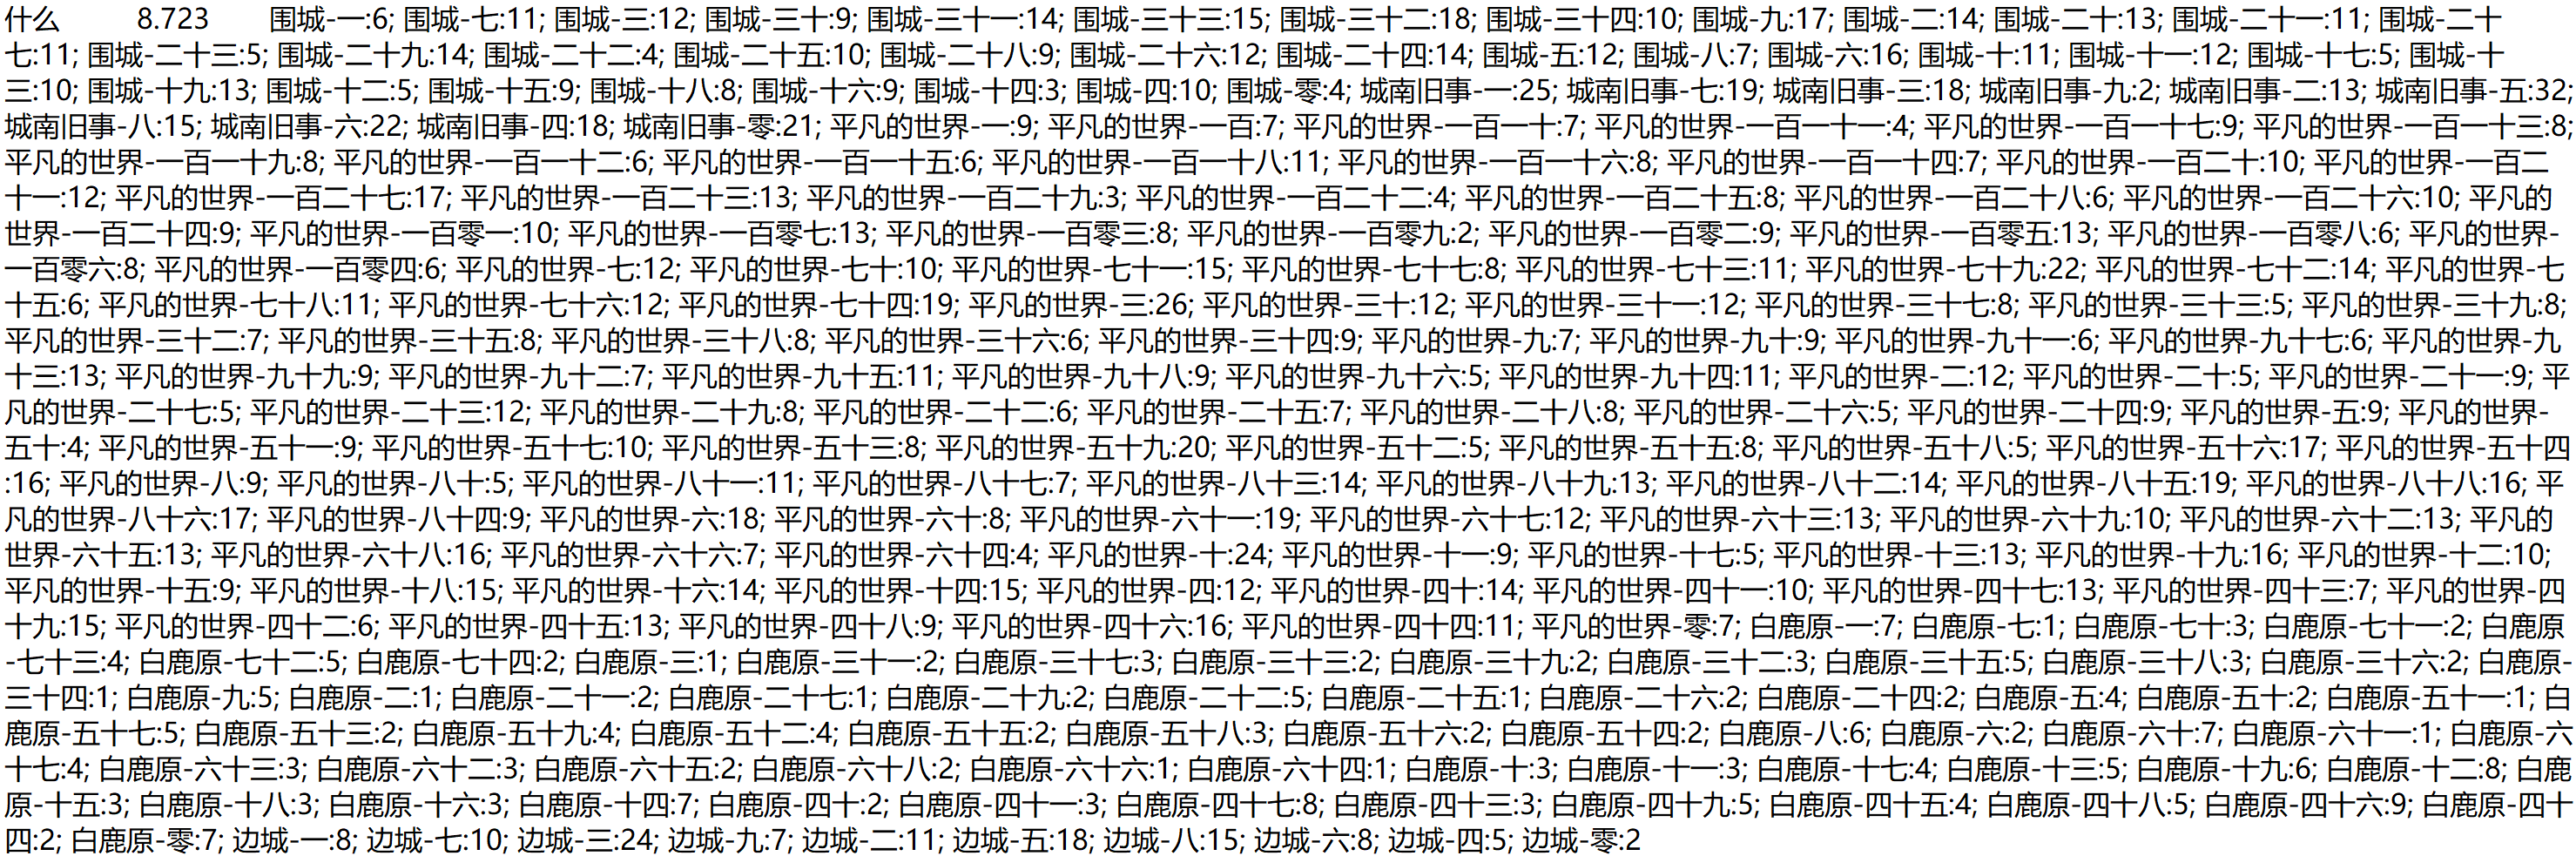
\includegraphics[scale=0.4]{./img/InvertedIndex_what.png}
	    \caption{基础功能-结果文件-“什么”}
	\end{figure} 
	\begin{figure}[H]
	    \centering
	    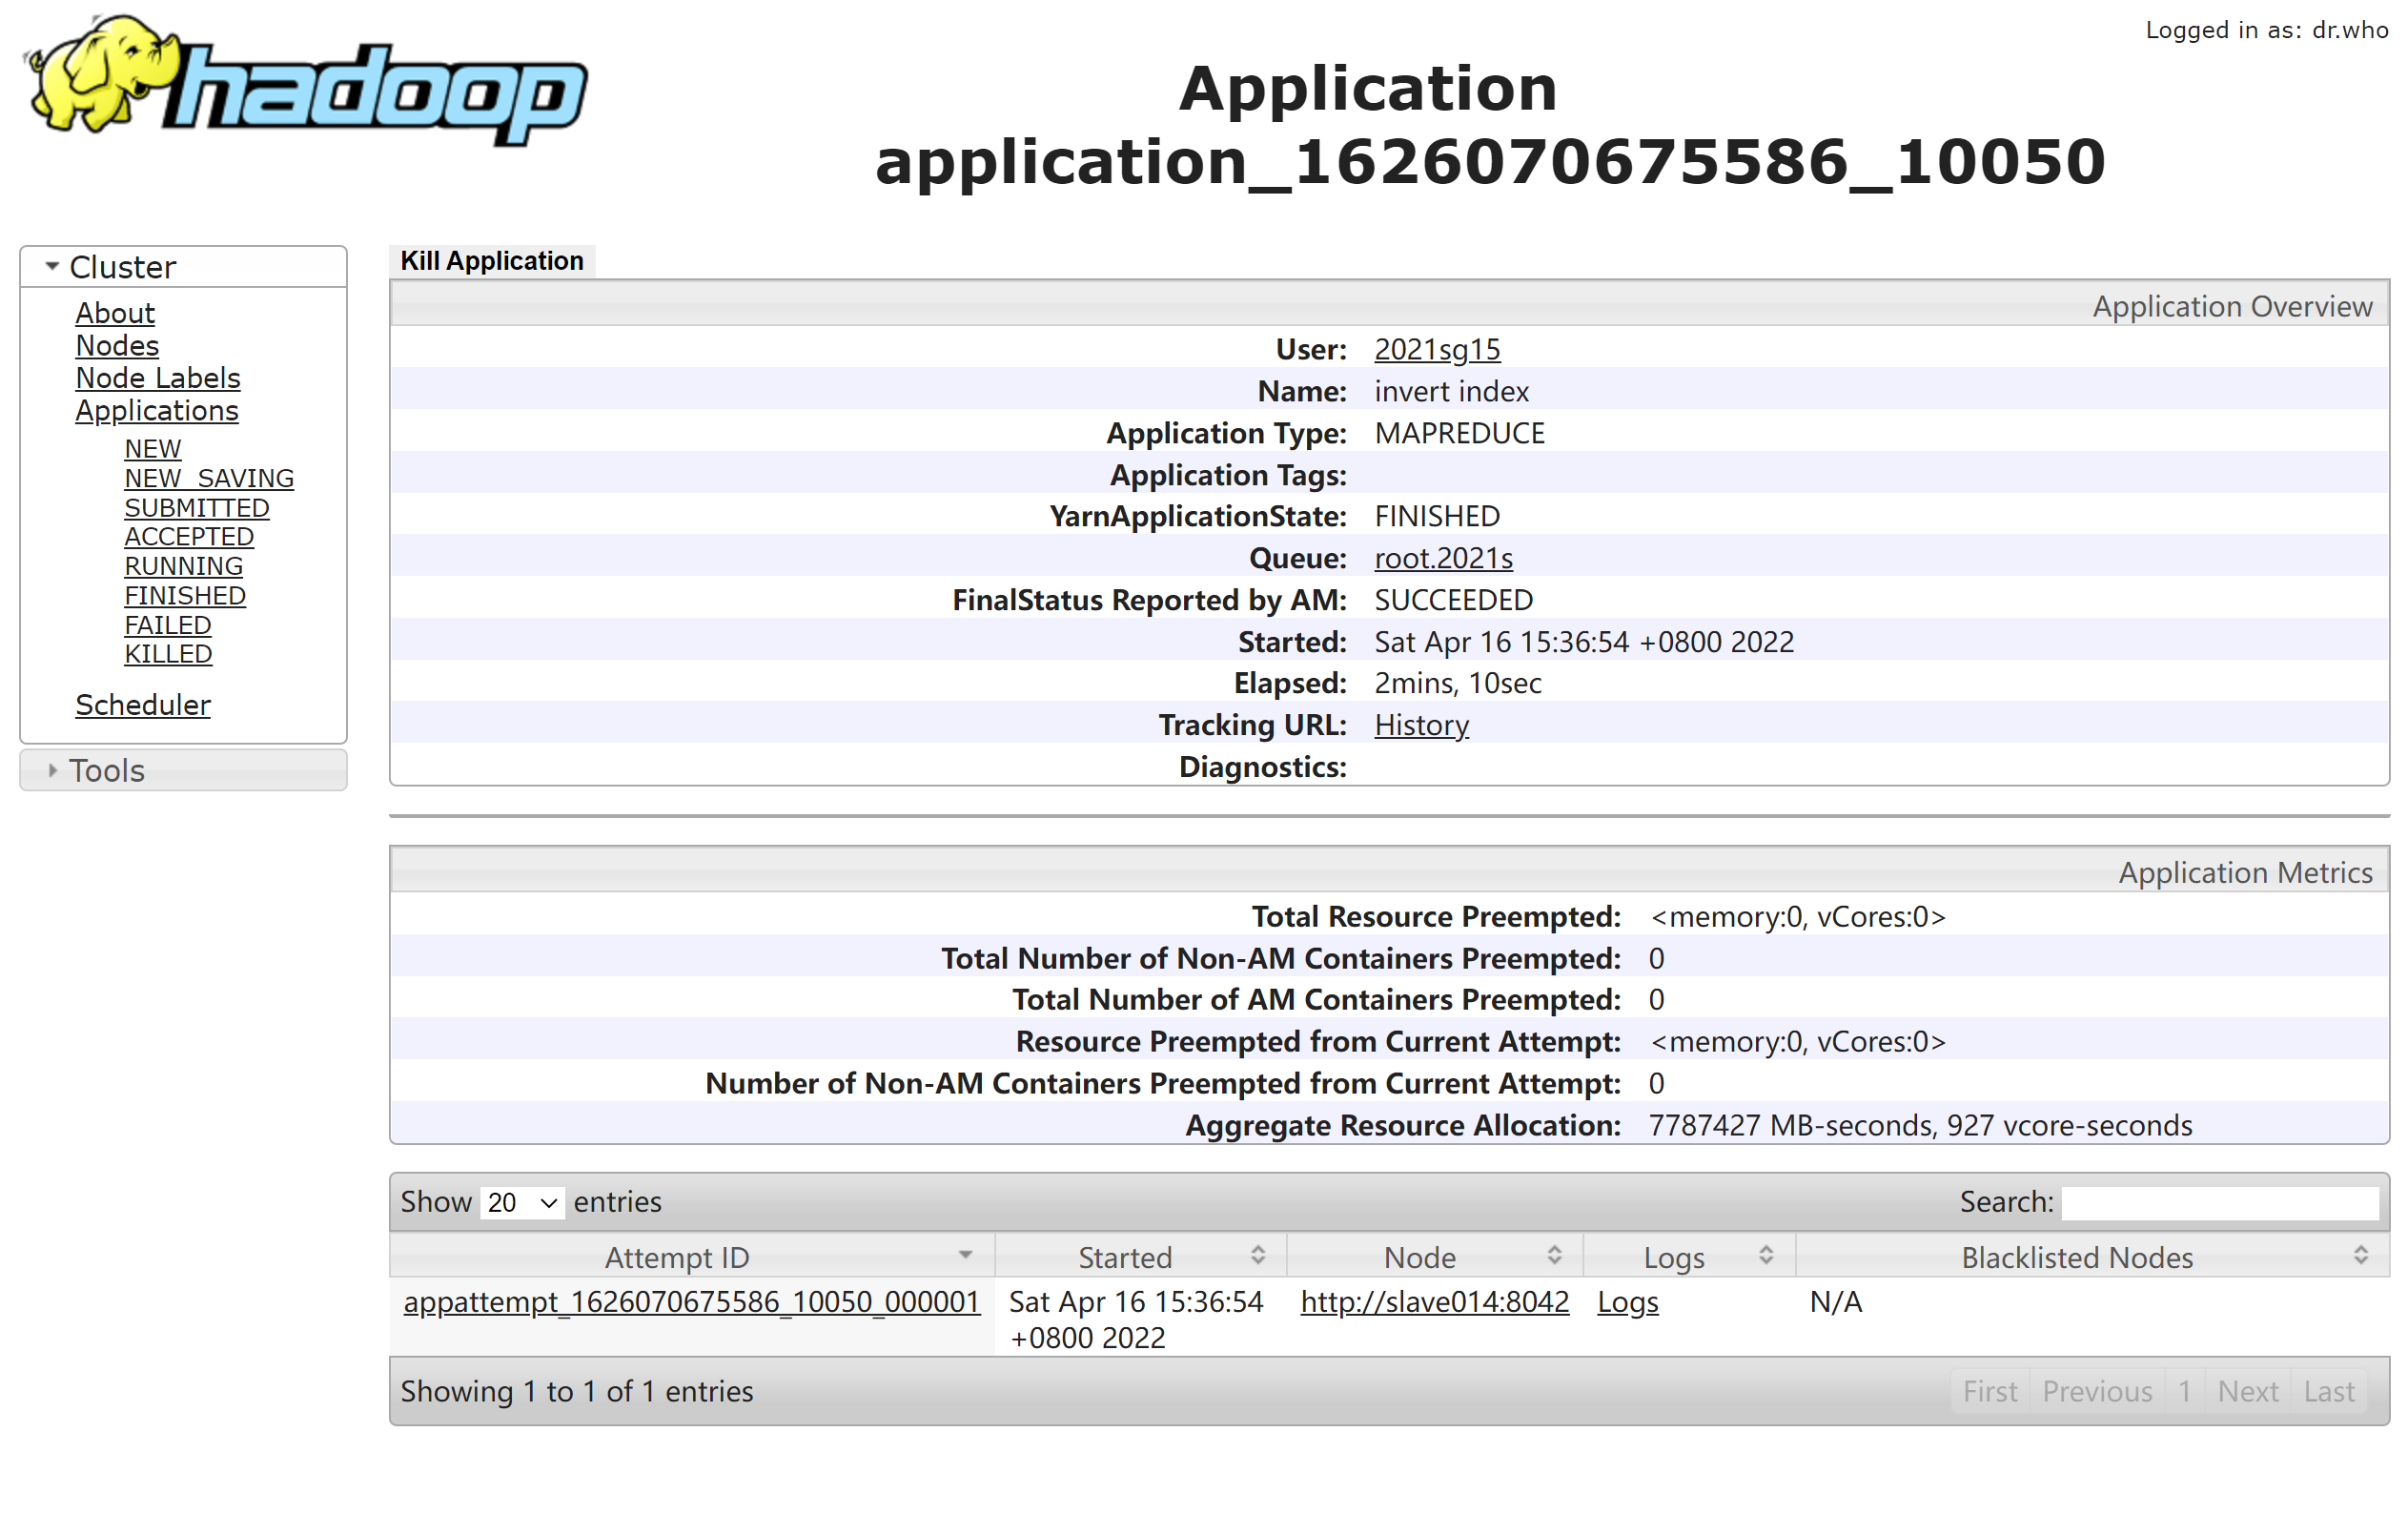
\includegraphics[scale=0.4]{./img/InvertedIndex.png}
	    \caption{基础功能-集群执行报告}
	\end{figure} 
	\item[2.] 选做1(排序)
	\par 输出文件路径:/user/2021sg15/lab2/out2
	\begin{figure}[H]
	    \centering
	    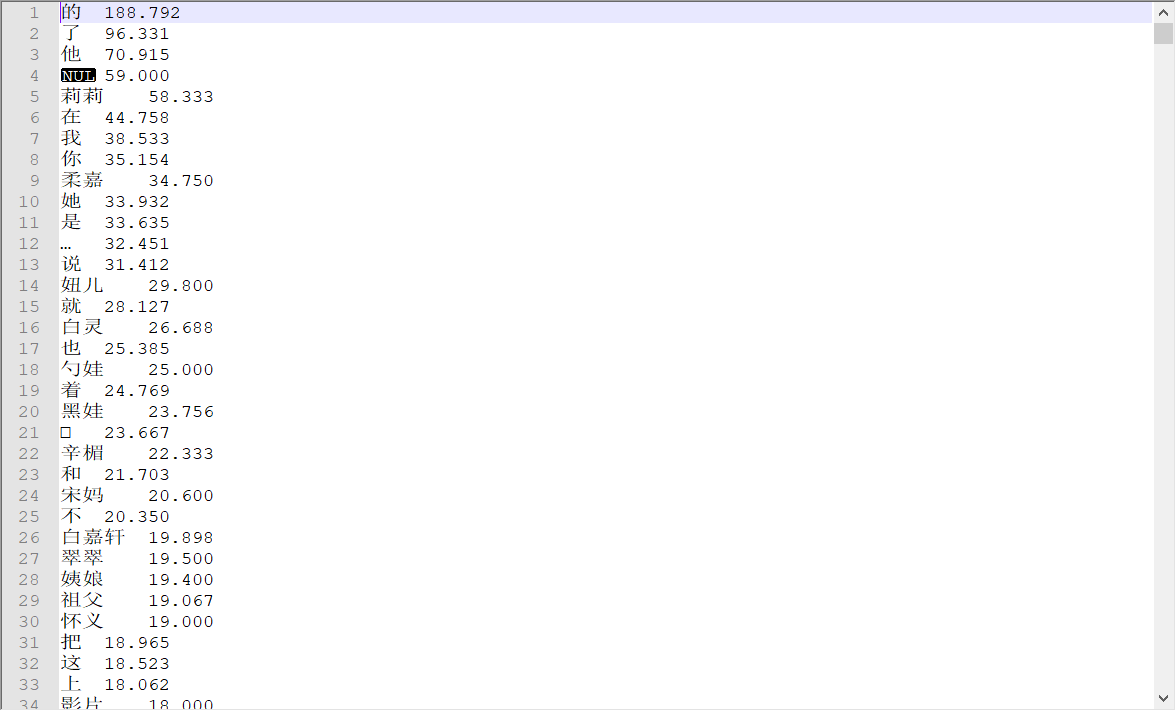
\includegraphics[scale=0.6]{./img/SortCount_res.png}
	    \caption{选做1(排序)-结果文件部分截图}
	\end{figure} 
	\begin{figure}[H]
	    \centering
	    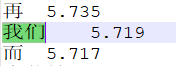
\includegraphics[scale=1.0]{./img/SortCount_we.png}
	    \caption{选做1(排序)-结果文件-“我们”}
	\end{figure} 
	\begin{figure}[H]
	    \centering
	    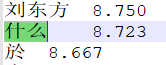
\includegraphics[scale=1.0]{./img/SortCount_what.png}
	    \caption{选做1(排序)-结果文件-“什么”}
	\end{figure} 
	\begin{figure}[H]
	    \centering
	    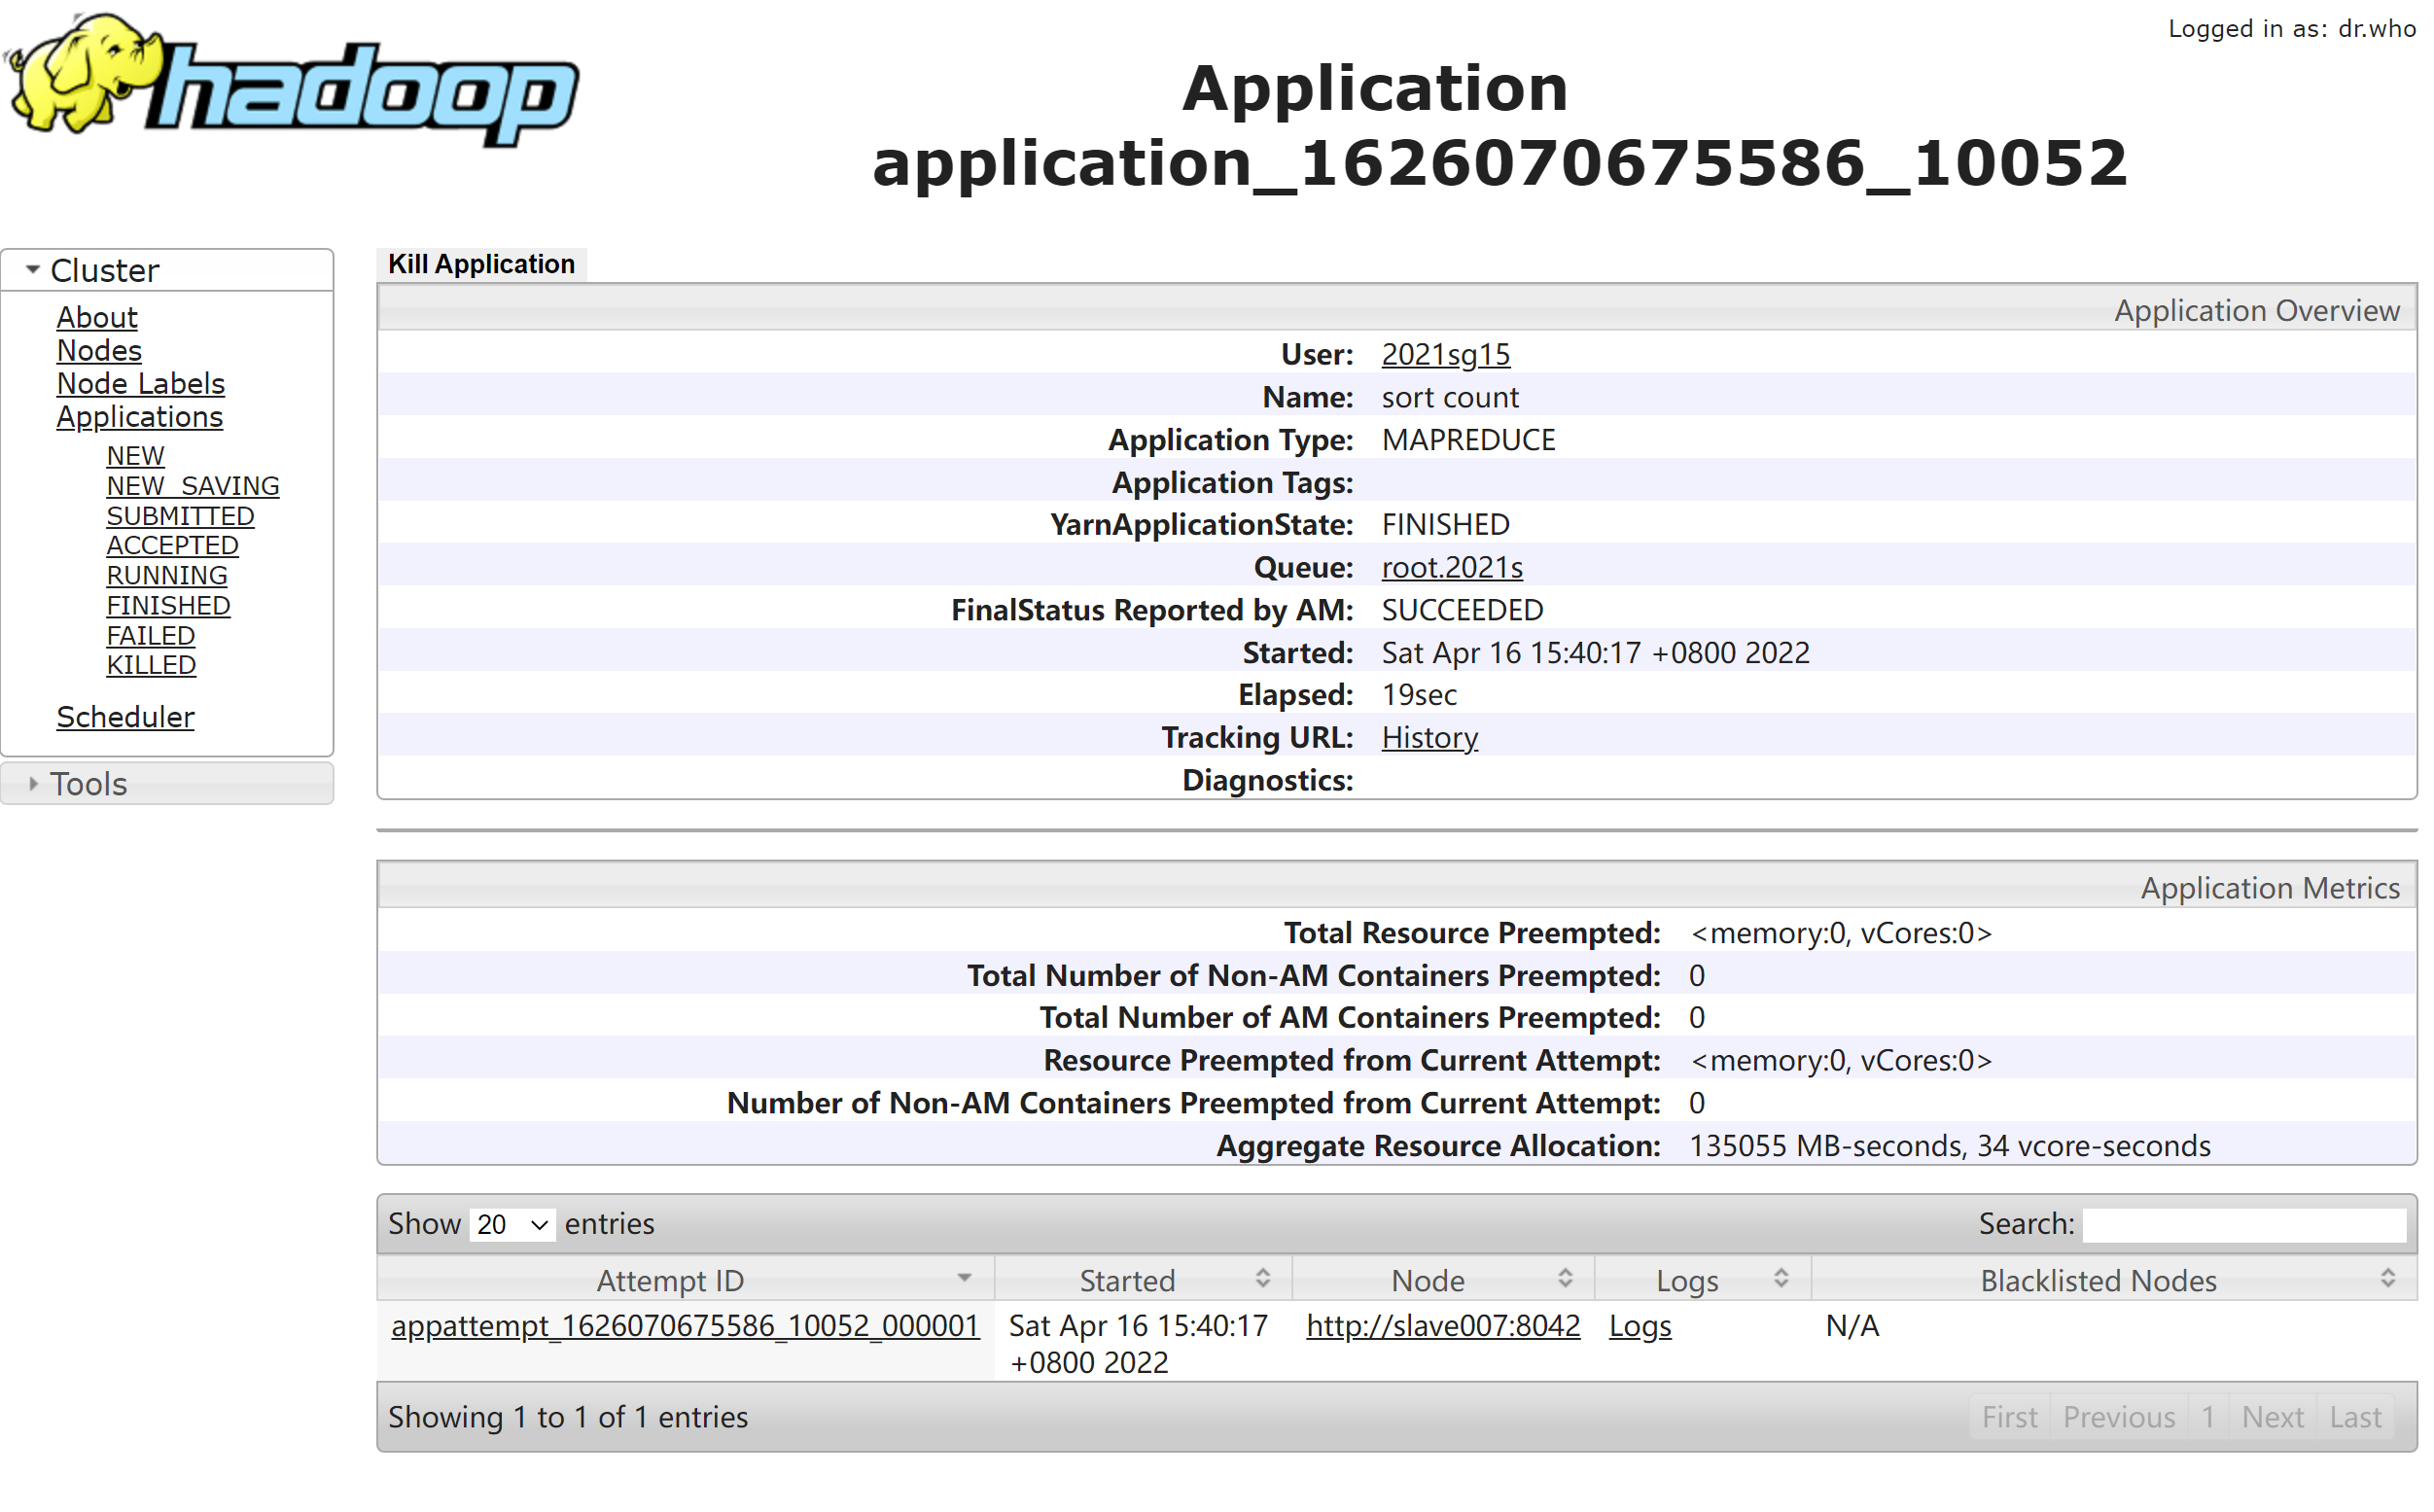
\includegraphics[scale=0.4]{./img/SortCount.png}
	    \caption{选做1(排序)-集群执行报告}
	\end{figure} 
	\item[3.] 选做2(TF-IDF)
	\par 输出文件路径:/user/2021sg15/lab2/out3
	\begin{figure}[H]
	    \centering
	    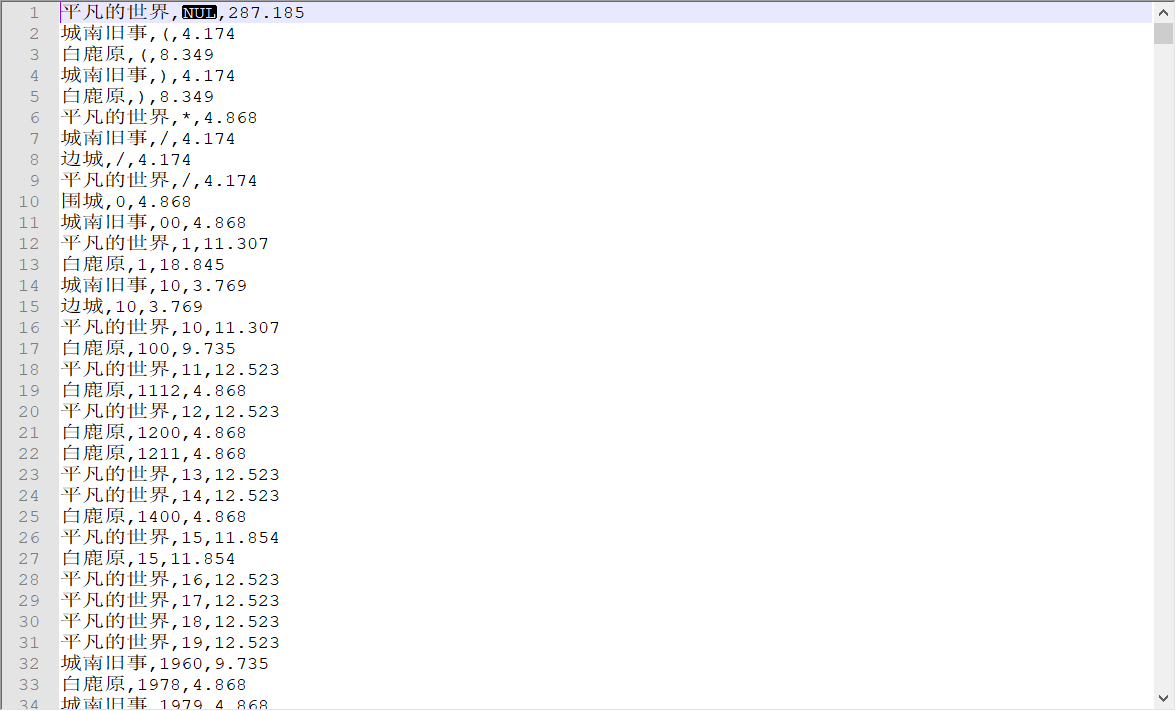
\includegraphics[scale=0.6]{./img/TFIDF_res.png}
	    \caption{选做2(TF-IDF)-结果文件部分截图}
	\end{figure} 
	\begin{figure}[H]
	    \centering
	    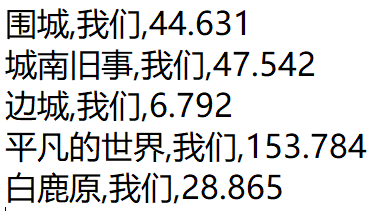
\includegraphics[scale=0.4]{./img/TFIDF_we.png}
	    \caption{选做2(TF-IDF)-结果文件-“我们”}
	\end{figure} 
	\begin{figure}[H]
	    \centering
	    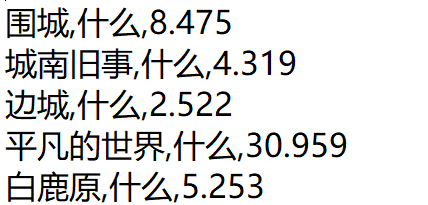
\includegraphics[scale=0.4]{./img/TFIDF_what.png}
	    \caption{选做2(TF-IDF)-结果文件-“什么”}
	\end{figure} 
	\begin{figure}[H]
	    \centering
	    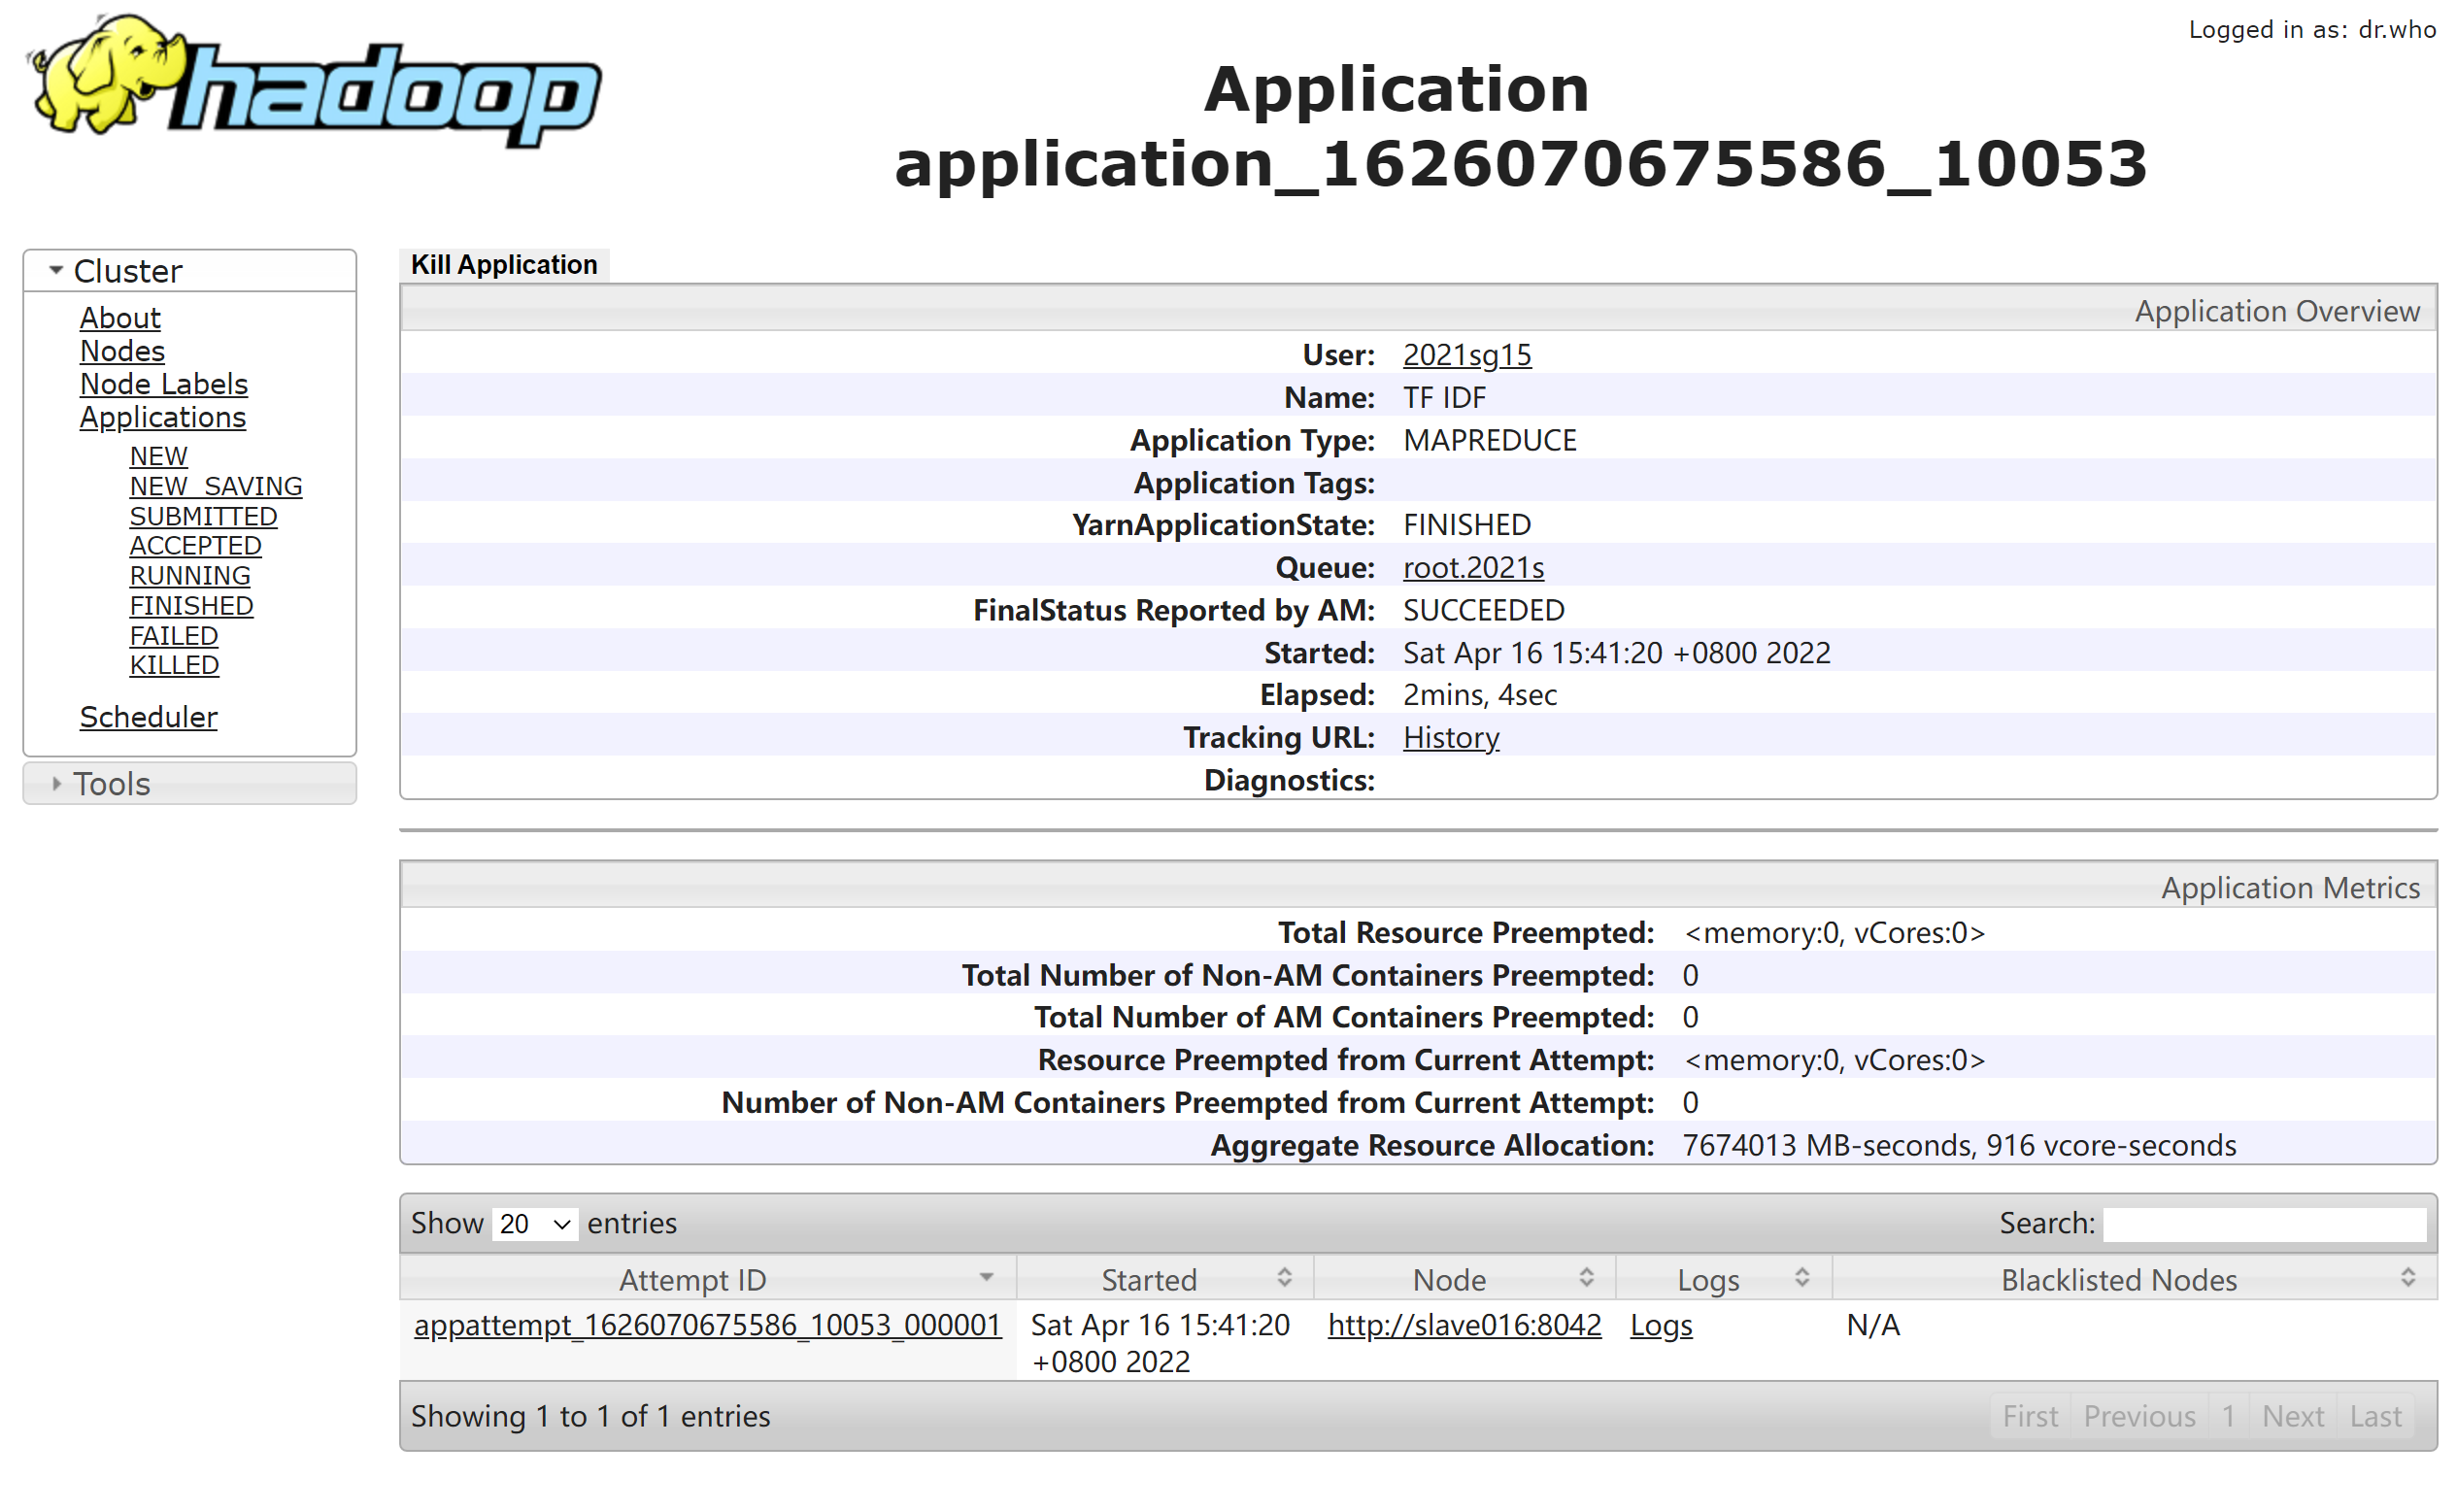
\includegraphics[scale=0.4]{./img/TFIDF.png}
	    \caption{选做2(TF-IDF)-集群执行报告}
	\end{figure} 
\end{enumerate}

\begin{CJK*}{UTF8}{gbsn}
\section*{三、基础功能}
\end{CJK*}
	\par \textbf{设计思路}
	\par Mapper类接受和发送的Key, Value类型:$<$Object, Text, Text, IntWritable$>$. 发送的key的含义是单词+文档名,发送的value的含义是key中单词在该文档的出现次数.这里需要重写Partitioner类,按照key中的单词作为划分标准.
	\par Reducer类接受和发送的Key, Value类型:$<$Text, IntWritable, Text, Text$>$. 包含当前单词的文档数的统计方法为:使用一个类成员变量$fileNumber$记录,在当前单词没有发生变化时自增1,否则在完成均值和倒排索引的计算后置0. 当前单词的总词频的计算方法为:在当前单词没有发生变化时,累加$values$中所有的值,同时在这一过程中使用StringBuiler记录当前文档的倒排索引及其词频.在当前词语发生变化时及完成所有项的统计后,计算均值并写出结果.
	\par \textbf{伪代码}

\begin{algorithm}[htb]
\caption{Mapper for InvertedIndexer}
\label{alg:Framwork}
\begin{algorithmic}[1] %这个1 表示每一行都显示数字
	 \STATE \textbf{method} Map(docid $dn$,doc $d$)
    \STATE Let $F$ be a new AssociatedArray.
    \FOR{each $t \in d$}
	 	\STATE $F\{t\} = F\{t\} + 1$;
	 \ENDFOR
    \FOR{each $t \in F$}
	 	\STATE $Emit(<t, docid>, F\{t\})$;
	 \ENDFOR
	 \RETURN
\end{algorithmic}
\end{algorithm}

\newpage
\begin{algorithm}[htb]
\caption{Reducer for InvertedIndexer}
\label{alg:Framwork}
\begin{algorithmic}[1] %这个1 表示每一行都显示数字
	 \STATE \textbf{method} Setup(docid $dn$,doc $d$)
	 \STATE $fileNumber$ := $0$;
	 \STATE $frequency$ := $0$;
	 \STATE $sumFrequency$ := $0$;
	 \STATE $t_{prev}$ := $\oslash$;
	 \STATE $P$ := new $PostingsList$;
	 \STATE 
    \STATE \textbf{method} $Reduce(<t, docid>, tf[])$
	 \IF {$t \neq t_{prev} \land t_{prev} \neq \oslash$}
		\STATE $average:=sumFrequency/fileNumber$;
	 	\STATE emit($prev, <average, P>$);
		\STATE $P$.reset();
		\STATE $fileNumber = 0$;
		\STATE $sumFrequency = 0$;
	 \ENDIF
	 \STATE $t_{prev} = t$;
	 \STATE $fileNumber = fileNumber + 1$;
	 \STATE $frequency = 0$;
	 \FOR {each $f \in tf$}
	 	\STATE $frequency = frequency + f$;
	 \ENDFOR
	 \STATE $sumFrequency = sumFrequency + frequency$;
	 \STATE $P$.add($<docid, frequency>$);
	\STATE
    \STATE \textbf{method} Close()
		\STATE $average:=sumFrequency/fileNumber$;
	 	\STATE emit($prev, <average, P>$);
	 \STATE
    \STATE \textbf{function} TF\_IDF(PostingsList$<docid, frequency>$ $P$, $IDF$, $word$)
	 \STATE res := new List;
	 \STATE $wordfile\_freq\_map$ := new AssociatedArray;
	 \STATE Let All elements in $wordfile\_freq\_map$ has default value $0$.
	 \FOR {each $<docid, frequency> \in P$}
		\STATE $fileName := docid$.substr$(0, docid.$indexOf$('-'))$;
		\STATE $wordfile\_freq\_map$[$fileName$] = $wordfile\_freq\_map$[$fileName$]$ + frequency$;
	 \ENDFOR
	 \FOR {each $<fileName, frequency>\in wordfile\_freq\_map$}
	 	\STATE $res$.add($<fileName, word, IDF*frequency>$);
	 \ENDFOR
	 \RETURN res;
\end{algorithmic}
\end{algorithm}
	
\begin{CJK*}{UTF8}{gbsn}
\section*{四、选做内容}
\end{CJK*}
\begin{enumerate}
	\item[A.] 排序出现次数的排序	\par \textbf{设计思路}
	\par 以基础功能的输出为输入:
	\par Mapper类接受和发送的Key, Value类型:$<$Object, Text, Text, Text$>$. 发送的value的含义是单词,发送的key的含义是该单词平均出现次数。重写WritableComparator的compare方法,以单词平均出现次数的降序进行排列。
	\par Reducer类接受和发送的Key, Value类型:$<$Text, Text, Text, Text$>$. 将得到的$<$value(单词)和key(平均出现次数)$>$作为输出。
	\par \textbf{伪代码}
\begin{algorithm}[htb]
\caption{Mapper for SortedCounter}
\label{alg:Framwork}
\begin{algorithmic}[1] %这个1 表示每一行都显示数字
	 \STATE \textbf{method} Map(docid dn, doc d)
    \STATE Let $F$ be a new AssociatedArray.
    \FOR{each $line <word, averageFrequency, postingList<docid, frequency>> \in d$}
	 	\STATE Emit$(averageFrequency, word)$;
	 \ENDFOR
	 \RETURN
\end{algorithmic}
\end{algorithm}
\begin{algorithm}[htb]
\caption{WritableComparator for SortedCounter}
\label{alg:Framwork}
\begin{algorithmic}[1] %这个1 表示每一行都显示数字
	 \STATE \textbf{method} Compare(WritableComparable a, WritableComparable b)
    \STATE Let double $m$ be the value of $a$.
 	\STATE Let double $n$ be the value of $b$.
	 \RETURN b.compareTo(a);
\end{algorithmic}
\end{algorithm}
\begin{algorithm}[htb]
\caption{Reducer for SortedCounter}
\label{alg:Framwork}
\begin{algorithmic}[1] %这个1 表示每一行都显示数字
	 \STATE \textbf{method} Reduce($frequency,words[]$)
	 \FOR{each $word \in words$}
		\STATE Emit($word, frequency$);
	 \ENDFOR
	 
\end{algorithmic}
\end{algorithm}
	\item[B.] 每个作品的每个词语的TF-IDF
	\par 
	\par \textbf{设计思路}
	\par Mapper类接受和发送的Key, Value类型:$<$Object, Text, Text, IntWritable$>$. 发送的key的含义是单词+文档名,发送的value的含义是key中单词在该文档的出现次数。这里需要重写Partitioner类,按照key中的单词作为划分标准。
	\par Reducer类接受和发送的Key, Value类型:$<$Text, IntWritable, Text, Text$>$. 语料库文档总数在main方法中由FileSystem获取,并存储在Configuration中. 在Reducer中通过上下文Context获取该项的值。包含当前单词的文档数的统计方法和基础功能中的实现相类似,这里不再赘述。得到了单词word对应的所有[文档-词频]以及该单词的IDF,遍历每个文档-词频计算其TF-IDF即可。注意对同一作品不同文档的词频求和才能得到正确的TF-IDF.
	\par \textbf{伪代码}

\begin{algorithm}[htb]
\caption{Mapper for TF-IDF}
\label{alg:Framwork}
\begin{algorithmic}[1] %这个1 表示每一行都显示数字
	 \STATE \textbf{method} Map(docid $dn$,doc $d$)
    \STATE Let $F$ be a new AssociatedArray.
    \FOR{each $t \in d$}
	 	\STATE $F\{t\} = F\{t\} + 1$;
	 \ENDFOR
    \FOR{each $t \in F$}
	 	\STATE $Emit(<t, docid>, F\{t\})$;
	 \ENDFOR
	 \RETURN
\end{algorithmic}
\end{algorithm}

\begin{algorithm}[htb]
\caption{Reducer for TF-IDF}
\label{alg:Framwork}
\begin{algorithmic}[1] %这个1 表示每一行都显示数字
	 \STATE \textbf{method} Setup(docid $dn$,doc $d$)
	 \STATE Let $srcFileCnt$ be the number of input files.
	 \STATE $fileNumber$ := $0$;
	 \STATE $frequency$ := $0$;
	 \STATE $t_{prev}$ := $\oslash$;
	 \STATE $P$ := new $PostingsList$;
	 \STATE $wordfile\_freq\_map$ := new AssociatedArray;
	 \STATE Let All elements in $wordfile\_freq\_map$ has default value $0$.
	 \STATE 
    \STATE \textbf{method} $Reduce(<t, docid>, tf[])$
	 \IF {$t \neq t_{prev} \land t_{prev} \neq \oslash$}
		\STATE $IDF := log(\frac{srcFileCnt}{fileNumber + 1})$;
		\STATE $wordfile\_freq\_map$.clear();
		 \FOR {each $<docid, frequency> \in P$}
			\STATE $fileName := docid$.substr$(0, docid.$indexOf$('-'))$;
			\STATE $wordfile\_freq\_map$[$fileName$] = $wordfile\_freq\_map$[$fileName$]$ + frequency$;
		 \ENDFOR
		 \FOR {each $<fileName, frequency>\in wordfile\_freq\_map$}
		 	\STATE Emit($<fileName, word>, IDF*frequency>$);
		 \ENDFOR
		\STATE $P$.reset();
		\STATE $fileNumber = 0$;
	 \ENDIF
	 \STATE $t_{prev} = t$;
	 \STATE $fileNumber = fileNumber + 1$;
	 \STATE $frequency = 0$;
	 \FOR {each $f \in tf$}
	 	\STATE $frequency = frequency + f$;
	 \ENDFOR
	 \STATE
	 \STATE $P$.add($<docid, frequency>$);
	\STATE
    \STATE \textbf{method} Close()
		\STATE $wordfile\_freq\_map$.clear();
		 \FOR {each $<docid, frequency> \in P$}
			\STATE $fileName := docid$.substr$(0, docid.$indexOf$('-'))$;
			\STATE $wordfile\_freq\_map$[$fileName$] = $wordfile\_freq\_map$[$fileName$]$ + frequency$;
		 \ENDFOR
		 \FOR {each $<fileName, frequency>\in wordfile\_freq\_map$}
		 	\STATE Emit($<fileName, word>, IDF*frequency>$);
		 \ENDFOR
    
\end{algorithmic}
\end{algorithm}
\end{enumerate}


\end{CJK}
\end{document}
